\documentclass[12pt]{article}
\usepackage[utf8]{inputenc}
\usepackage{amsmath,amssymb}
\usepackage{unicode-math}
\usepackage[T2A]{fontenc}
\usepackage[russian]{babel}
\usepackage{graphicx}
\usepackage{subfigure}
\usepackage{subcaption}
\usepackage{url}


\DeclareGraphicsExtensions{.pdf,.png,.jpg}
\usepackage{hyperref}
\usepackage{wrapfig}
\usepackage[left=20mm, top=20mm, right=10mm, bottom=20mm]{geometry}

\usepackage{amsmath} 
\usepackage{amsfonts} 
\usepackage{amssymb} 
\usepackage{wasysym} 
\usepackage{fancyhdr}

\pagestyle{fancy}
\fancyhf{}
\lhead{Семинары 4 и 5. Уравнение Шредингера. Ямы и барьеры}
\rhead{\textit{Клименок К.Л., МФТИ 2020}}
\rfoot{\thepage}



\begin{document} 
\title{\textbf{Семинары 4 и 5. Волновая функция, потенциальные ямы и барьеры. Уравнение Шредингера}}
\author{\textbf{Клименок Кирилл Леонидович}}
\date{24.09.2020}
\maketitle

\section{Теоретическая часть}
Для начала --- небольшой дисклеймер. Объединение этих двух семинаров произошло, потому что все задачи, которые необходимо решить в них, относятся, по сути, к уравнению Шредингера, методикам его решения и следствиям из него. 

\subsection{Волновая функция}
На прошлой неделе мы с вами уже поняли, что такое корпускулярно-волновой дуализм, и даже выписали соотношение неопределённостей. Но это, скорее, было выведено умозрительно и на пальцах. Сейчас мы поговорим о математическом представлении этого дела. Мы знаем, как связаны импульс частицы и ее длина волны: $p  = \hbar k = \dfrac{h}{\lambda}$\vspace{1mm}, и энергия частиты и её частота: $E  = \hbar \omega$. Теперь запишем некоторую плоскую волну и, вместо волнового вектора и частоты, подставим импульс и энергию. Это и будет волна де Бройля для нашей частицы:
\begin{equation}
\label{eq:sem_04_psi}
    \psi = \psi_0 \exp{\left[i\left(kx - \omega t \right)\right]} =\psi_0 \exp{\left[\dfrac{i}{\hbar}\left(px - Et \right)\right]}
\end{equation}
То есть, это такой аналог плоской волны в оптике, но не для электромагнитных волн, а для частиц. Как мы помним из курса оптики, такие плоские волны это математическая абстракция, с которой нам очень удобно работать, но в реальности их не существует (такая волна должна бежать из бесконечности в бесконечность и обладать бесконечной энергией), поэтому вопроса коэффициента и нормировки этой волны не стоит. 

Продолжим обсуждать физический смысл такой волновой функции для частицы. Здесь нам продолжают помогать аналогии из курса волновой оптики. Когда мы решали задачи на интерференцию и дифракцию, мы говорили, что мы можем детектировать не амплитуду волны, а интенсивность --- её квадрат. Так вот, в квантовой механике всё точно так же. Сама $\psi$-функция  не несет в себе явного физического смысла, в отличие от её квадрата, который говорит нам о плотности вероятности найти частицу в заданном диапазоне параметров. Этот факт мы неявно рассматривали на прошлом семинаре, когда говорили об эксперименте Hitachi.  Отсюда у нас появляется первый ряд свойств $\psi$-функции:
\begin{itemize}
    \item $\psi$-функция непрерывна. Если бы у функции существовал разрыв, то вероятность найти частицу в точке разрыва была бы разной.
    \item Квадрат $\psi$-функции нормируется на 1, как и любая другая функция плотности вероятности. Мы же точно найдем нужную нам частицу в бесконечном пространстве вселенной? $$\int\psi^*\psi dV = 1$$
\end{itemize}
Небольшой комментарий о принципе суперпозиции. Здесь он работает как простое суммирование вероятностей, и квадраты коэффициентов разложения нашей общей $\psi$-функции здесь являются простыми вероятностями найти частицу в данном состоянии (для любителей строгой математики: $\psi$-функции разных состояний ортогональны, и когда считают полную вероятность, их перекрестные произведения обращаются в ноль).

\subsection{Операторы физических величин. Уравнение Шредингера}
Хорошо, мы более-менее осознали формализм нашей волновой функции и поняли, что она значит. Но как тогда описывать поведение частиц, которые описываются волновыми функциями? И самый главный вопрос: как тогда переходить к обычным и привычным параметрам описания системы из классической механики, где нет никаких вероятностей, а есть конкретный электрон в конкретном месте на экране?

Для начала определимся с понятием состояния нашей частицы или системы частиц. В классике все было просто: была конкретная координата, конкретный импульс, и всё. В квантах у нас есть некоторые <<сцепленные>> между собой параметры, и тогда состояние --- это конкретные значения только независимых из них и все множество возможных значений других параметров.

Хорошо, а как нам тогда это описывать? Вот тут понадобится немного математики. В классике, при переходе из состояния с координатой $r_1$ в состояние с координатой $r_2$ появлялась функция $r(t)$, которая всё и показывала. Что же будет в квантах? Есть состояние $\psi_1$, которое описывается функцией, и состояние $\psi_2$, которое описывается другой функцией. Тогда при переходе из одного состояния в другое должна быть функция от функции, которая и будет заниматься этим переводом. Такая конструкция называется оператором.

Какими свойствами должны обладать операторы? Во-первых, из-за принципа суперпозиции они должны быть линейными. Во-вторых, раз уж мы хотим как-то связать оператор физической величины с самой измеряемой величиной, то просто договоримся, что собственные числа нашего оператора соответствуют измеряемым в эксперименте значениям.

Теперь получим сами операторы, с которыми будем иметь дело. Все операторы обозначаются <<крышечкой>>. Для начала, если посмотреть на (\ref{eq:sem_04_psi}), то мы увидим связанные между собой $x$ и $p$. Значит, в зависимости от того, что мы выберем: импульс или координату, изменятся и наши операторы. В нашем курсе мы работаем исключительно с координатным представлением, и оператор координаты тогда будет просто умножать нашу $\psi$-функцию на координату:
\begin{equation}
\label{eq:sem_04_coordinate}
    \hat{x}\psi = x\psi
\end{equation}

Как получить из нашей волновой функции (\ref{eq:sem_04_psi}) импульс? Достаточно просто продифференцировать ее с правильным коэффициентом:
\begin{gather}
\label{eq:sem_04_momentum}
    \hat{p_x}\psi = -i\hbar\dfrac{\partial\psi}{\partial x} = p_x \psi\\
    \hat{\textbf{p}}\psi = -i\hbar\nabla\psi = \textbf{p} \psi
\end{gather}

Ещё нам будет нужен оператор полной энергии, или оператор Гамильтона. Он состоит из операторов кинетической и потенциальной энергии $\hat{T}$ и $\hat{U}$:
\begin{equation}
\label{eq:sem_04_hamilton}
    \hat{H}\psi = \hat{T}\psi + \hat{U}\psi = \dfrac{\hat{p}^2}{2m}\psi + \hat{U}\psi = -\dfrac{\hbar^2}{2m}\left(\dfrac{\partial^2}{\partial x^2} + \dfrac{\partial^2}{\partial y^2} + \dfrac{\partial^2}{\partial z^2}\right)\psi + U(x,y,z)\psi = -\hbar^2\Delta\psi + U(x,y,z)\psi
\end{equation}

В данном выражении возведение оператора импульса в квадрат эквивалентно его двойному применению, символ $\Delta$ --- оператор Лапласа. Поскольку потенциальная энергия зависит только от координат, ее оператор ведет себя также как и оператор координаты (\ref{eq:sem_04_coordinate}). 

Таким образом, если система находится в стационарном состоянии, то для того, чтобы найти её энергию, нужно просто подействовать оператором Гамильтона на нашу $\psi$-функцию и получить все возможные значения уровня энергии. Это уравнение и называется стационарным уравнением Шредингера:
\begin{equation}
\label{eq:sem_04_schrodinger}
    \hat{H}\psi = E\psi
\end{equation}

В нестационарном случае, энергию можно получить напрямую из волновой функции (\ref{eq:sem_04_psi}) с помощью дифференцирования по времени. Такой оператор называют оператором эволюции. Это --- нестационарное уравнение Шредингера:
\begin{equation*}
    i\hbar\dfrac{\partial\psi}{\partial t} = \hat{H}\psi
\end{equation*}

Выводя все эти операторы, мы наткнулись ещё на одно свойство волновой функции, а именно ее гладкость. Почему это так важно? Если наша функция не гладкая, то при действии оператора импульса появляется скачок импульса. А что по физике это означает? Только наличие бесконечной силы. В реальном мире такого нет, есть только в модельных задачах, одну из которых мы решим позднее.

И прежде, чем двигаться дальше, небольшая ремарка о средних значениях разных физических величин. На самом деле, ничего принципиально сложного в этом нет. В рамках курса общей физики мы говорили о расчете средних значений ещё на термодинамике, а потом это должно было повторяться и на теории вероятностей. Чтобы посчитать среднее значение оператора, достаточно правильно свернуть его с нашей отнормированной волновой функцией:
\begin{equation*}
    \langle A\rangle = \int\psi^*\hat{A}\psi dV
\end{equation*}

\subsection{Задачи о барьерах}
В этом разделе мы посмотрим, как с помощью уравнения Шредингера можно решить задачу о налетании частицы на барьер. 
\paragraph{Одномерная ступенька}
Рассмотрим задачу об обычном одномерном барьере: таком, что $\,U_I(x) = 0,\; x<0$ и $U_{II}(x) = U,\; x \geqslant 0$. Пусть поток частиц летит из области отрицательных координат с энергией $E<U$. Нам с помощью стационарного уравнения Шредингера надо найти волновые функции частицы из такого потока, а также узнать что у нее с отражением от описанного барьера. Тут сразу в глаза бросается, что происходит что-то не то. В классике такая частица не может существовать под барьером: просто не проходит по энергиям. А вот в квантовом мире это уже не так очевидно. Поэтому давайте запишем волновые функции для каждой из областей и посмотрим, что и как происходит, записав уравнение Шредингера.
\begin{gather*}
    \begin{cases}
         \dfrac{\hbar^2}{2m}\dfrac{\partial^2\psi_1}{\partial x^2} +  E\psi_1=0; &x<0  \\[10pt]
         \dfrac{\hbar^2}{2m}\dfrac{\partial^2\psi_2}{\partial x^2} - (U - E)\psi_2=0; &x \ge 0
    \end{cases}
\end{gather*}
\begin{figure}[h]
    \centering
    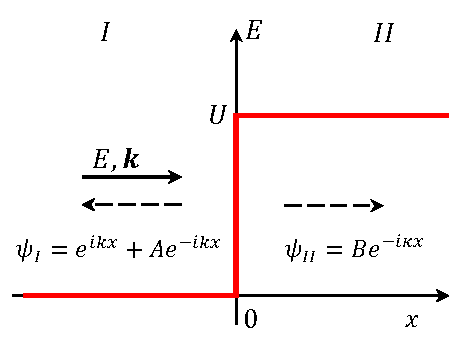
\includegraphics[width=0.7\textwidth,height=\textheight,keepaspectratio]{Seminar_04/pics/pic_01.pdf}
    \caption{Структура потенциала одномерного бесконечного барьера и волновые функции частиц.}
    \label{fig:sem_04}
\end{figure}

Ясно, что решить такое после курса дифференциальных уравнений вы в состоянии\vspace{2mm}, поэтому ограничусь тем, что скажу, что в первой области введем число $k = \sqrt{\dfrac{2mE}{\hbar^2}}$, а во второй $ \kappa = \sqrt{\dfrac{2m(U -E)}{\hbar^2}}$. Тогда решения с учетом произвольных постоянных будут записаны как
\begin{gather*}
    \begin{cases}
         \psi_1(x) = e^{ikx} + A e^{-ikx}; &x<0  \\
         \psi_2(x) = Be^{-\kappa x}; &x\ge 0  
    \end{cases}
\end{gather*}

Здесь мы исключили растущую экспоненту во второй области из физических соображений, весь входящий поток частиц отнормировали на 1. Решение с плюсом и минусом в области $x<0$ соответствует частицам, которые бегут к и от барьера. Остались только коэффициенты $A$ и $B$, которые можно спокойно найти из условия сшивки волновых функций на границе в точке $x=0$, тогда 
\begin{gather*}
    \begin{cases}
        A = \dfrac{1 - i\kappa/k}{1 + i\kappa/k}\\[5pt]
        B = \dfrac{2}{1 + i\kappa/k}
    \end{cases}
\end{gather*}

Казалось бы, все прекрасно, получили решение, но вот незадача: сумма квадратов наших коэффициентов не дает 1. Это означает, что мы где-то потеряли какую-то вероятность. На самом деле, так и должно быть, ведь нормировка такой волновой функции подразумевает бесконечную вероятность из-за расходимости в отрицательной области. Это мы уже обсуждали с вами в первой части семинара. Как же тогда получить что-то физически адекватное? Нужно от волновой функции перейти к потоку вероятности. Идея вывода потока вероятности совпадает с выводом обычного потока частиц из термодинамики: выделяем объем $dV$, из которого за время $dt$ налетают на барьер частицы с известными нам волновыми функциями, и считаем их вероятность найтись в этом объеме:
\begin{gather*}
    dV = \dfrac{p}{m}dtdS = \dfrac{\hbar k}{m}dtdS\\
    dw = \psi^2dV = \psi^2\dfrac{\hbar k}{m}dtdS = \textbf{j}dtdS
\end{gather*}

$\textbf{j}$ здесь и несет в себе смысл потока вероятности,  и именно на него и надо смотреть при обсуждении вопроса о прозрачности барьера, а не на исходные коэффициенты в решении для $\psi$-функции. Окончательно, если мы говорим о проницаемости и отражательной способности барьера, мы смотрим именно на отношение потоков прошедшего и отраженного к исходному, и там уже сумма квадратов дает адекватный результат, сумма которого равна 1:
\begin{gather*}
    T = \dfrac{j_{\text{прош}}}{j_{\text{пад}}} = \dfrac{\kappa B^2}{k} = \dfrac{4k\kappa}{(k+\kappa)^2} \\
    R = \dfrac{j_{\text{отр}}}{j_{\text{пад}}} = \dfrac{k A^2}{k} = \dfrac{(k-\kappa)^2}{(k+\kappa)^2}
\end{gather*}

\paragraph{Одномерный барьер. Туннелирование}
Тут все почти как и в предыдущем случае, но в отличие от бесконечной ступеньки, здесь барьер имеет конечную ширину $a$. 

\begin{figure}[h]
    \centering
    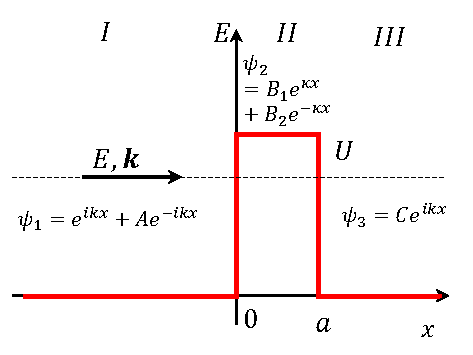
\includegraphics[width=0.7\textwidth,height=\textheight,keepaspectratio]{Seminar_04/pics/pic_02.pdf}
    \caption{Структура потенциала одномерного бесконечного барьера и волновые функции частиц.}
    \label{fig:sem_04}
\end{figure}

\vspace{2mm}
Опять вводим числа $k = \sqrt{\dfrac{2mE}{\hbar^2}}$ и $ \kappa = \sqrt{\dfrac{2m(U -E)}{\hbar^2}}$, а решение ищем в виде
\begin{gather*}
    \begin{cases}
         \psi_1(x) = e^{ikx} + A e^{-ikx}; &x<0  \\
         \psi_2(x) = B_1e^{\kappa x} + B_2e^{-\kappa x}; & a\le x\ge 0  \\
         \psi_3(x) = Ce^{ikx} ; &x>a  \\
    \end{cases}
\end{gather*}

Здесь мы забиваем по физическому смыслу только на волну, которая бежит налево в области $x>a$. Дальше, как и в предыдущем случае, сшиваем решение по непрерывности и гладкости в $x=0$ и $x=a$:
\begin{gather*}
    \begin{cases}
         1+A = B_1+B_2  \\
         ik(1-A) = B_1-B_2 \\
         Ce^{ika} = B_1e^{\kappa a} + B_2e^{-\kappa a}\\
         ikCe^{ika} = \kappa (B_1e^{\kappa a} - B_2e^{-\kappa a})\\
    \end{cases}
\end{gather*}

Дальше --- небольшая магия математики и расчета потока вероятности для того, чтобы найти коэффициент прохождения через барьер:
\begin{gather*}
        D = \dfrac{j_{\text{прош}}}{j_{\text{пад}}} = \dfrac{k C^2}{k} = \dfrac{4k^2\kappa^2}{4k^2\kappa^2 + (k^2+\kappa^2)^2 \sh^2{\kappa a}} = \dfrac{4k^2\kappa^2}{4k^2\kappa^2 + \dfrac{2mU}{\hbar^2} \sh^2{\kappa a}}
\end{gather*}

Основной физический смысл такого результата заключается в том, что частица с некоторой вероятностью может пролететь сквозь барьер, который запрещен для нее классической физикой. Обсудим некоторые следствия из этой формулы. Там правда есть всякие забавности и неочевидности.

\paragraph{Предельные случаи}
Их, как обычно, 2: или барьер очень узкий/невысокий ($\kappa a \ll 1$), или обратное, когда барьер высокий/широкий ($\kappa a \gg 1$). Очевидно, что это будет влиять только на разложение гиперболического синуса в формуле и тогда будем иметь:
\begin{gather*}
    D \approx \dfrac{1}{1 + \dfrac{(k^2+\kappa^2)^2}{4k^2}a^2}, \; \kappa a \ll 1\\
    D \approx \dfrac{4k^2\kappa^2}{(k^2+\kappa^2)^2}e^{-2\kappa a} \approx e^{-2\kappa a}, \; \kappa a \gg 1
\end{gather*}

И если первое выражение нам не особенно интересно, то второй предельный случай нужен, чтобы получить приближенную формулу для произвольного барьера

\paragraph{Барьер произвольной формы}
Что будем делать если барьер задан какой-то функцией $U(x)$. Есть первый вариант: решить уравнение Шредингера честно. Скажу сразу: вариант очень на любителя, так как это почти никогда не работает. Как упростить беде жизнь? Разбить наш барьер на множество маленьких прямоугольных барьерчиков, забить на переотражение между ними и использовать готовое решение из предельного случая:
\begin{gather}
\label{eq:sem_04_tunnel_coeff}
    D \approx \prod\limits_{i} D_i \approx \prod\limits_{i} e^{-2\kappa_i dx_i} = \exp{\left( -2\sum\limits_{i}\kappa_i dx_i \right)} = \exp{\left( -2\int\limits_{0}^{a}\sqrt{\dfrac{2m(U(x)-E)}{\hbar^2}} dx \right)}
\end{gather}

Интегрирование здесь ведется только по классически запрещенной области.

\paragraph{Надбарьерное отражение}
Окей, а что изменится в квантовом описании, если энергия частицы будет больше, чем высота барьера? В классике, такая частица просто не заметила бы его и пролетела дальше. В квантовом мире это не так, и есть вероятность, что частица отразится от барьера. Естественно, перерешивать всю задачу снова мы не будем, а воспользуемся готовым решением, с той лишь разницей, что $E>U$. Тогда  всё, что изменится в нашем решении, это $\kappa = ik_2$ и тогда в коэффициенте прохождения гиперболический синус изменится на обычный (а еще немного поплывут знаки):
\begin{gather*}
        D =  \dfrac{4k^2k_2^2}{4k^2k_2^2 + (k^2-k_2^2)^2 \sin^2{k_2 a}}
\end{gather*}

То есть, коэффициент прохождения будет равен 1 только тогда, когда синус в знаменателе обратится в 0, то есть на ширине барьера будет укладываться целое число полуволн: $k_2 a = \pi n$.

\textit{Комментарий:} вообще-то все это прекрасно работает и для потенциальных ям, только там $U$ меняется на $-U$, но выводы те же самые. Такое явление полного пропускания частиц с определенными длинами волн называется эффектом Рамзауэра.

\subsection{Задачи о ямах}
\paragraph{Одномерная яма с бесконечными стенками}
С потенциалом такой ямы все максимально просто:
\begin{gather*}
    U(x) = \begin{cases}
         \infty, &x<0 \text{ или } x>a \\
          0, &0<x<a 
    \end{cases}
\end{gather*}
\begin{figure}[h]
    \centering
    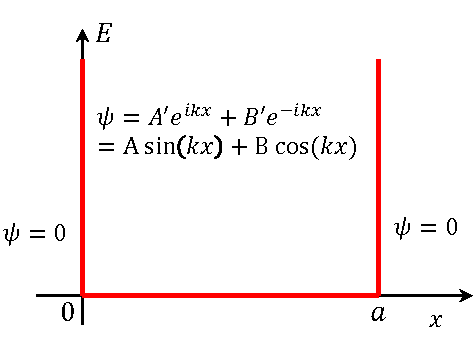
\includegraphics[width=0.7\textwidth,height=\textheight,keepaspectratio]{Seminar_04/pics/pic_03.pdf}
    \caption{Структура потенциала одномерной ямы с бесконечными стенками и волновые функции частицы в ней}
    \label{fig:sem_04_1D_inf_hole}
\end{figure}

Но предположение о бесконечных стенках не слишком физичное. Из-за этого мы должны, во-первых, сказать, что частица локализована в именно в яме, а ее волновая функция снаружи равна нулю, а, во-вторых, на границах ямы мы должны отказаться от гладкости.

Теперь давайте запишем уравнение Шредингера и найдем все возможные волновые функции частиц в яме:
\begin{gather*}
    \begin{cases}
         \dfrac{\hbar^2}{2m}\dfrac{\partial^2\psi}{\partial x^2} +  E\psi=0; &a>x>0  \\[10pt]
         \psi=0;  &x<0 \text{ или } x>a 
    \end{cases}
\end{gather*}

Ну а с решением здесь все максимально просто. Ищем его в виде синуса и косинуса с какими-то коэффициентами и сшиваем. Из-за того что $\psi(0) = 0$, косинус откидываем, и останется стандартное условие, что на длине ямы должно укладываться целое число полуволн:
\begin{gather}
\label{eq:sem_04_energy_in_hole}
    \begin{cases}
         \psi_n(x) = A_n \sin(k_nx)\\
         k_na = \pi n\\[5pt]
         E_n = \dfrac{\hbar^2k_n^2}{2m} = \dfrac{\hbar^2\pi^2n^2}{2ma^2}
    \end{cases}
\end{gather}
где коэффициент $A_n$ можно найти из нормировки. Самый главный вывод из этого всего заключается в том, что теперь в яме частица может занимать не любые уровни энергии, а только конкретные с определенной энергией. Это будет работать и в общем случае, а не только для такой модельной ямы. Примерами этого может служить электрон в атоме водорода, колеблющаяся двухатомная молекула и другие объекты, которые бы будем рассматривать.

\paragraph{Примеры реальных ям, их потенциалы и уровни энергии}
Вот несколько оговоренных примеров. Честное решение этих задач будет приведено в курсе теоретической физики, здесь же мы ограничимся простым формулированием ответа.

\vspace{3mm}
\noindent
\textit{\textbf{Гармонический осциллятор}} 
\begin{gather*}
    U(x) = \dfrac{m\omega^2x^2}{2}\\
    E_n(x) = \hbar\omega(n+\dfrac{1}{2}); n\ge 0
\end{gather*}

\noindent
\textit{\textbf{Электрон в атоме водорода}} 
\begin{gather*}
    U(r) = -\dfrac{e^2}{r}\\
    E_n(x) = -\dfrac{R_H}{n^2}; n\ge 1; R_H = 13.6 \text{ эВ} 
\end{gather*}

\paragraph{Квазиклассическое приближение}
Кажется, что такая модельная задача про бесконечно глубокую яму вообще нужна исключительно как иллюстрация того, как запудить мозги хорошим людям на квантах. Но это не так! Идея использования такой ямы как раз и нужна для оценки уровней энергии в разных сложных потенциалах.
\begin{figure}[h]
    \centering
    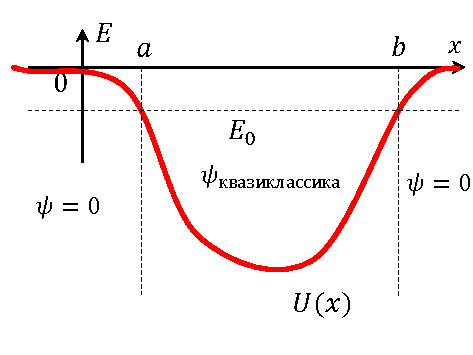
\includegraphics[width=0.7\textwidth,height=\textheight,keepaspectratio]{Seminar_04/pics/pic_04.pdf}
    \caption{Квазиклассическое приближение}
\end{figure}

Пусть у нас есть какая-то яма $U(x)$, и в ней живет частица с какой-то энергией $E$ достаточно далеко от дна ямы. Это нужно для того, чтобы мы могли не париться о том, что происходит в классически запрещенной области и сказали, что там, как и у ямы с бесконечными стенками, волновая функция примерно 0. Тогда в классически разрешенной области мы от $a$ до $b$ (это так называемые <<точки поворота>>) должны решать уравнение Шредингера:
\begin{gather*}
    \begin{cases}
         \dfrac{\hbar^2}{2m}\dfrac{\partial^2\psi}{\partial x^2} +  (E-U(x))\psi=0; &b>x>a  \\[10pt]
         \psi=0;  &x<a \text{ или } x>b 
    \end{cases}
\end{gather*}

И тогда мы просто можем заменить $U(x)$ на яму с бесконечными стенками с шириной $b-a$. Пока звучит очень так себе, но с примерами все станет понятно.

Рассмотрим всё ту же параболическую яму из примера выше. Определим ширину ямы: она будет $2x_m$, где $\pm x_m$ это точки поворота, и $E = \dfrac{m\omega^2x_m^2}{2}$. Выразим $x_m$ через энергию: $x_m=\sqrt{\dfrac{2E}{m\omega^2}}$. Теперь подставим это в \ref{eq:sem_04_energy_in_hole}:
\begin{gather*}
    E = \dfrac{\pi^2\hbar^2n^2}{2m(2x_m)^2 } = \dfrac{\pi^2\hbar^2n^2 m\omega^2}{16mE  } \\
    E = \dfrac{\pi}{4}\hbar\omega n
\end{gather*}

Видно, что качественно мы получили тот же результат, что и в строгой теории (эквидистантные уровни энергии), но с  небольшим поправочным множителем. Этот подход несколько более общий и позволяет рассчитывать и волновые функции, но на нем мы останавливаться не будем. Такого понимания на мой взгляд будет достаточно.



\section{Практическая часть}
\subsection{Задача 3.4}
\label{task_3.4}
\paragraph{Условие}
Волновая функция частицы массой $m$, совершающей одномерное движение в поле с потенциалом $U(x)$, есть 
\begin{gather*}
\psi(x) = 
    \begin{cases}
        Ax\exp{\left( -\dfrac{x}{a}\right)}; &x \ge 0\\
        0; &x<0
    \end{cases}
\end{gather*}
Оценить с помощью соотношения неопределенностей среднюю кинетическую энергию $\langle T \rangle$ частицы и сравнить с результатом точного расчета. Найти среднее значение координаты $\langle x \rangle$, а также $U(x)$ при $x>0$ и полную энергию $E$, если известно, что $U(x) \rightarrow 0$ при $x \rightarrow \infty$.

\paragraph{Решение}
Эта задача на игры с волновой функцией и понимание того, как считать средние значения операторов.

Начнем с чего попроще, а именно с плотности вероятности найти частицу:
\begin{gather*}
    w(x) = \psi^*\psi = A^2x^2\exp{\left( -\dfrac{2x}{a}\right)} \text{ при }  x \ge 0
\end{gather*}

Явно видно, что при малых $x$ функция растет, а при больших --- убывает, значит есть определенный максимум, который можно посчитать:
\begin{gather*}
    \dfrac{dw(x)}{dx} = 0 \Rightarrow x_m = a
\end{gather*}

Тогда мы можем оценить неопределенность по координате как $2a$ --- влево и вправо от максимума. Тогда, из соотношения неопределенностей:
\begin{gather*}
    p \approx \Delta p = \dfrac{\hbar}{2a} \Rightarrow \langle T \rangle = \dfrac{p^2}{2m} = \dfrac{\hbar^2}{8ma^2}
\end{gather*}

Теперь найдем среднее значение координаты честно, опустив интегрирование:
\begin{gather*}
    \langle x \rangle = \dfrac{\int\limits_0^{\infty}\psi(x)^*x\psi(x)dx}{\int\limits_0^{\infty}\psi(x)^*\psi(x)dx} = \dfrac{3a}{2}
\end{gather*}

Далее найдем полную энергию и потенциал, подставив в уравнение Шредингера известную нам волновую функцию:
\begin{gather*}
    \dfrac{\hbar^2}{2m}\dfrac{\partial^2\psi}{\partial x^2} +  (E-U(x))\psi=0\\
    U(x) - E = \dfrac{\hbar}{2max}\left( \dfrac{x}{a} - 2 \right)
\end{gather*}

Из условия, что на бесконечности потенциал равен нулю, находим энергию:
\begin{gather*}
    E = -\dfrac{\hbar^2}{2ma^2}
\end{gather*}

И, зная это, находим потенциал:
\begin{gather*}
    U(x) = - \dfrac{\hbar^2}{max}
\end{gather*}

То есть, это обычный кулоновский потенциал.

\subsection{Задача 3.34}
\label{task_3.34}
\paragraph{Условие}
Электрон находится в основном состоянии в одномерной потенциальной яме и имеет энергию $E = 1.5$ эВ. Ширина ямы равна $9a = 3 \cdot 10^{-8}$ см. Найти высоту потенциального барьера $U$ и его проницаемость $D$. За какое время $\tau$ вероятность найти частицу в яме уменьшится в два раза? Отражением волновой функции на задней границе потенциального барьера пренебречь.
\begin{figure}[h]
    \centering
    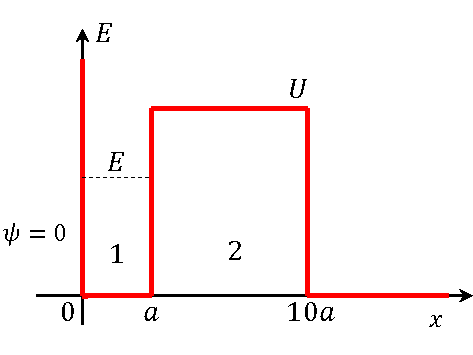
\includegraphics[width=0.6\textwidth,height=\textheight,keepaspectratio]{Seminar_04/pics/pic_05.pdf}
    \caption{Рисунок к задаче 3.34}
\end{figure}

\paragraph{Решение}
Ну, тут опять нужно аккуратно составить уравнение Шредингера и решить его для областей 1 и 2, обозначенных на рисунке. Единственное отличие от теоретической части --- это упрощение, связанное с отсутствием отражения от задней стенки. Что это означает, будет ясно из решения. 

Итак, запишем уравнение Шредингера в областях 1 и 2:
\begin{gather*}
    \begin{cases}
         \dfrac{\hbar^2}{2m}\dfrac{\partial^2\psi_1}{\partial x^2} +  E\psi_1=0; &a>x>0  \\[10pt]
         \dfrac{\hbar^2}{2m}\dfrac{\partial^2\psi_2}{\partial x^2} - (U - E)\psi_2=0; & 10a>x>a
    \end{cases}
\end{gather*}
Как и раньше, обозначим $k = \sqrt{\dfrac{2mE}{\hbar^2}}$ и $ \kappa = \sqrt{\dfrac{2m(U -E)}{\hbar^2}}$. Понятно, что в первой области будут синусы и косинусы, а во второй экспоненты. Но, учитывая отсутствие отражения от стенки $10a$, растущей экспоненты во 2 области не будет:
\begin{gather*}
    \begin{cases}
         \psi_1(x) = A \sin{kx} + B \cos{kx}\\
         \psi_2(x) = Ce^{-\kappa x} 
    \end{cases}
\end{gather*}

Дальше давайте сшивать решения и находить коэффициенты. Первое: в нуле бесконечная стенка, за ней волновая функция ноль, сшивка только по непрерывности. Отсюда сразу понятно, что $B=0$, так косинус в $x=0$ не 0. Второе: непрерывность в $x=a$. Третье: гладкость там же:
\begin{gather*}
    \begin{cases}
         A \sin{ka} = Ce^{-\kappa a} \\
         Ak \cos{ka} = -C\kappa e^{-\kappa a}
    \end{cases}
\end{gather*}

Отсюда вытащим тангенс и попытаемся через него выразить высоту барьера:
\begin{gather*}
    \tan{ka} = -\dfrac{k}{\kappa}= - \sqrt{\dfrac{E}{U-E}} \Rightarrow U-E = \dfrac{E}{\tan^2{ka}} \Rightarrow U = E(1 + \dfrac{1}{\tan^2{ka}}) = \dfrac{E}{\sin^2{ka}}
\end{gather*}

Теперь мы сможем все честно посчитать и получим $U = 1.64$ эВ. Что с проницаемостью барьера? Для этого найдем $\kappa =1.92\cdot 10^7 \text{ см}^{-1}$, а проницаемость найдем в приближении широкого барьера: $D = \exp{\left( -2\kappa(10a-a)\right)} = 3.2\cdot10^{-5}$.
Теперь давайте оценим время уменьшения концентрации частиц вдвое. С каждым ударом о стенку для частицы есть вероятность $D$ покинуть яму. Тогда вероятность остаться в яме это $1-D$, и ее нужно просто возвести в степень числа ударов о стенку и приравнять к $1/2$. Пусть $n=\dfrac{v}{2a}$ -- частота ударов о стенку, тогда:
\begin{gather*}
    (1-D)^{n\tau} = \dfrac{1}{2}\\
    \tau = \dfrac{\ln{2}}{nD} = 1.8\cdot 10^{-11} \text{ c}
\end{gather*}

\subsection{Задача 3.40}
\label{task_3.40}
\paragraph{Условие}
В 1988 г. появилось сенсационное сообщение о осуществлении холодного ядерного синтеза дейтерия, растворенного в металлическом палладии. Можно считать, что при этом ядра дейтерия взаимодействуют друг с другом по закону Кулона, если расстояние между ними $r$ удовлетворяет условию $R_1 = 2\cdot 10^{-13} \text{ см} \le r \le  R_2 = 5\cdot 10^{-9} \text{ см}$. При большем расстоянии между ядрами энергия электрического отталкивания $U=0$ за счет экранирования ядер дейтерия электронами проводимости. Определить вероятность реакции синтеза $d+d$\; при столкновении дейтронов внутри палладия при комнатной температуре за счет туннельного эффекта. Считать, что реакция синтеза происходит при $r<R_1$.
\begin{figure}[h]
    \centering
    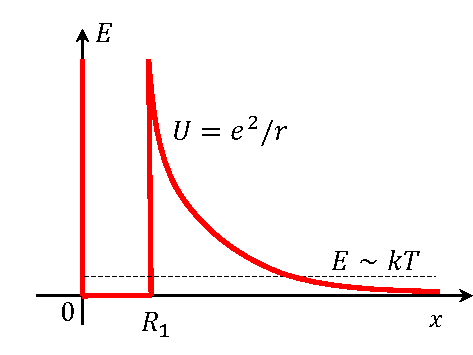
\includegraphics[width=0.6\textwidth,height=\textheight,keepaspectratio]{Seminar_04/pics/pic_06.pdf}
    \caption{Рисунок к задаче 3.40}
\end{figure}
\paragraph{Решение}
Задачка опять про туннелирование под кулоновским барьером. Нам, по сути, нужно оценить вероятность такого туннелирования --- и всё, даже уравнение Шредингера писать не надо. Для вероятности туннелирования у нас есть известная формула \ref{eq:sem_04_tunnel_coeff}, которой мы и воспользуемся. Только давайте определимся, что туда подставлять. Энергия частицы это $E = kT$ для комнатной температуры. Потенциал ---
%поколдовать с vspace'ами
 $U(r) = \dfrac{e^2}{r}$ --- обычный кулоновский потенциал. Границы интегрирования --- это те места, где $E=U(r)$, причем из-за малости $R_1$ мы вообще можем забить на нее и сказать, что это 0. Теперь найдем $R_2' = \dfrac{e^2}{kT} \approx 10^{-6} \text{ см}$. Это означает, что кинетическая энергия частицы настолько мала, что нам придётся в качестве верхнего предела брать именно $R_2$ из условия. 
\begin{gather*}
     D  = \exp{\left( -2\int\limits_{0}^{R_2}\sqrt{\dfrac{2m(e^2/r-kT)}{\hbar^2}} dr \right)} = \exp{\left( -\dfrac{2e}{\hbar}\sqrt{2mR_2} \right)} \approx e^{-235} \approx 0
\end{gather*}

Как мы видим, это событие довольно маловероятное.

\subsection{Задача a-la 3.14}
\label{task_3.14}
\paragraph{Условие}
Поток нейтронов падает на длинную щель с абсолютно отражающими стенками. При какой минимальной скорости нейтроны смогут пройти через эту щель?
\begin{figure}[h]
    \centering
    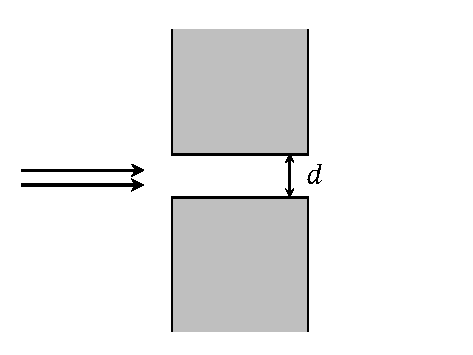
\includegraphics[width=0.3\textwidth,height=\textheight,keepaspectratio]{Seminar_04/pics/pic_07.pdf}
    \caption{Рисунок к задаче 3.14}
\end{figure}
\paragraph{Решение}
Если бы нейтроны были частицами, они бы прошли щель без проблем. Но если щель маленькая, то нейтроны мы можем рассматривать как волны, поэтому уместно вспомнить волновод. Как показывалось в курсе электричества, не всякая волна может войти в волновод. Здесь, по сути, все точно так же, только вместо электромагнитной волны у нас будет волна де Бройля. Тогда щель для нейтронов выступает в роли ямы с бесконечными стенками. Следовательно, для нейтрона возникают уровни энергий. Следовательно, если энергия нейтрона равна энергиям этих уровней, то нейтрон в щель войдет, и там навсегда останется. То есть, его компонента скорости вдоль начального направления будет нулевая. Если энергия больше, то нейтрон пройдет через эту щель:
\begin{gather*}
    \dfrac{mv^2}{2} > E_{n=1} = \dfrac{\pi^2\hbar^2}{2md^2}
\end{gather*}

\subsection{Комментарии к задачам из задания}
\paragraph{Нулевки 4 недели} Задачки на подстановку в формулы из теории.

\paragraph{Нулевки 5 недели} Задачки на формулу для энергии частицы в яме с бесконечными стенками.

\paragraph{Задача 3.5} Записать уравнение Шредингера и использовать известную волновую функцию для расчета энергии.

\paragraph{Задача 3.6} Использовать как пример расчет в квазиклассическом приближении из теоретической части. Правило квантования Бора-Зоммерфельда интерпретировать как интеграл по импульсу от 0 до $x$ и обратно.

\paragraph{Задача 3.14} Использовать идеи из \ref{task_3.14}.

\paragraph{Задача 3.21} Честно решить уравнение Шредингера и честно посчитать коодинату как в \ref{task_3.4}.

\paragraph{Задача 3.27} Комбинация идей из последнего параграфа из барьеров в расчетах вероятности как в \ref{task_3.34}.

\paragraph{Задача 3.28} Решить уравнение Шредингера в сферически симметричном случае (переведите лапласиан в сферические координаты, подгон волновой функции для решения: $\psi(r) = \dfrac{A}{r}\sin{kr}$). Запишите полную энергию с учетом поверхностного натяжения, найдите минимум.

\paragraph{Задача 3.33} Эффект Рамзауэра обсуждался в теоретической части.

\paragraph{Задача 3.40} Решена.

\paragraph{Задача 3.41} Задача уровня <<подставь в формулу>>.

\paragraph{Задача 3.45} Коэффициент отражения по мощности, тот, который из потока вероятности.

\paragraph{Задача 3.49} Нужно немного исследовать решение для ямы конечной ширины и посмотреть, что там будет. В качестве стартовой точки имеет смысл глянуть лекцию Глазкова или вывести все самостоятельно.

\paragraph{Задача T-1} Задачка уровня <<исследуй квадрат волновой функции, полученной в семинаре>>.

\end{document}
